\chapter{Plan działania}
\label{chap:czwarty}

\section{Wprowadzenie}
Celem projektu jest stworzenie aplikacji, która będzie dostępna w trzech wersjach:
\begin{itemize}
    \item Aplikacja internetowa (wersja dla administratorów i klientów),
    \item Aplikacja mobilna dla kierowców,
    \item Aplikacja mobilna dla klientów.
\end{itemize}

Każda z tych wersji będzie miała unikalne funkcjonalności dostosowane do specyfiki użytkowników.

\section{Plan działania}
\subsection{Etapy prac}
\begin{enumerate}
    \item \textbf{Analiza wymagań:}
    \begin{itemize}
        \item Zdefiniowanie grup docelowych.
        \item Identyfikacja kluczowych funkcji dla każdej wersji aplikacji.
    \end{itemize}
    \item \textbf{Projektowanie interfejsu:}
    \begin{itemize}
        \item Przygotowanie makiet dla aplikacji internetowej.
        \item Projektowanie interfejsów mobilnych dla aplikacji kierowców i klientów.
    \end{itemize}
    \item \textbf{Implementacja:}
    \begin{itemize}
        \item Budowa aplikacji internetowej w React.
        \item Tworzenie aplikacji mobilnych z wykorzystaniem React Native.
        \item Integracja z backendem (np. Node.js, Firebase).
    \end{itemize}
    \item \textbf{Testowanie:}
    \begin{itemize}
        \item Testy jednostkowe i integracyjne.
        \item Testy użyteczności dla każdej wersji aplikacji.
    \end{itemize}
    \item \textbf{Wdrożenie:}
    \begin{itemize}
        \item Publikacja aplikacji mobilnych w sklepach (Google Play, App Store).
        \item Wdrożenie aplikacji internetowej na serwer produkcyjny.
    \end{itemize}
    \item \textbf{Utrzymanie i rozwój:}
    \begin{itemize}
        \item Monitorowanie działania aplikacji.
        \item Wdrażanie nowych funkcji na podstawie opinii użytkowników.
    \end{itemize}
\end{enumerate}

\subsection{Harmonogram}
\begin{tabular}{|l|l|}
    \hline
    \textbf{Etap} & \textbf{Termin realizacji} \\
    \hline
    Analiza wymagań & 2 tygodnie \\
    \hline
    Projektowanie interfejsu & 3 tygodnie \\
    \hline
    Implementacja & 8 tygodni \\
    \hline
    Testowanie & 4 tygodnie \\
    \hline
    Wdrożenie & 2 tygodnie \\
    \hline
\end{tabular}

\section{Mapa aplikacji}
Poniżej przedstawiono strukturę aplikacji w postaci drzewa:

\begin{center}
    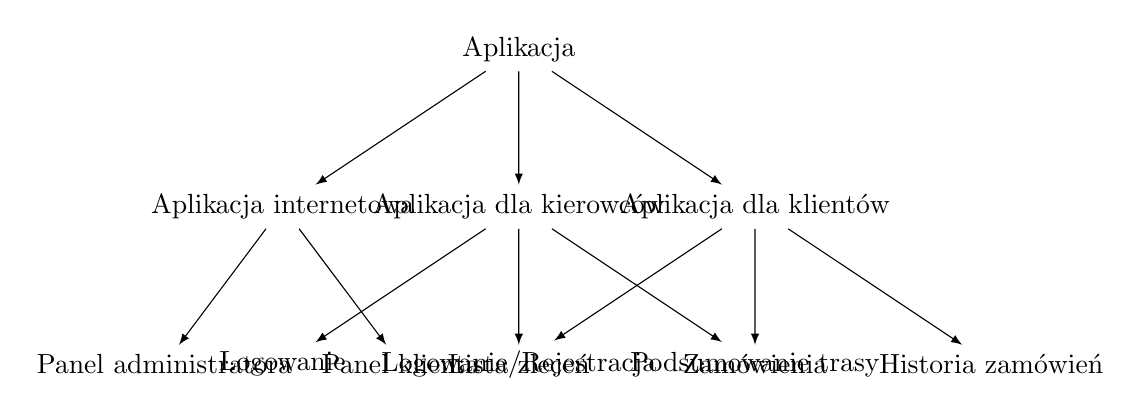
\begin{tikzpicture}[level distance=2cm, sibling distance=3cm, edge from parent/.style={draw,-latex}]
        \node {Aplikacja}
            child { node {Aplikacja internetowa}
                child { node {Panel administratora} }
                child { node {Panel klienta} }
            }
            child { node {Aplikacja dla kierowców}
                child { node {Logowanie} }
                child { node {Lista zleceń} }
                child { node {Podsumowanie trasy} }
            }
            child { node {Aplikacja dla klientów}
                child { node {Logowanie/Rejestracja} }
                child { node {Zamówienia} }
                child { node {Historia zamówień} }
            };
    \end{tikzpicture}
\end{center}

\section{Technologie}
\begin{itemize}
    \item \textbf{Frontend:} React, React Native.
    \item \textbf{Backend:} Node.js, Express, Firebase.
    \item \textbf{Bazy danych:} Firebase Firestore, PostgreSQL.
    \item \textbf{Inne:} Docker, CI/CD (GitHub Actions, Jenkins).
\end{itemize}